\documentclass[border=10pt]{standalone}
\usepackage{tikz}
\usetikzlibrary{arrows.meta, calc}

\begin{document}
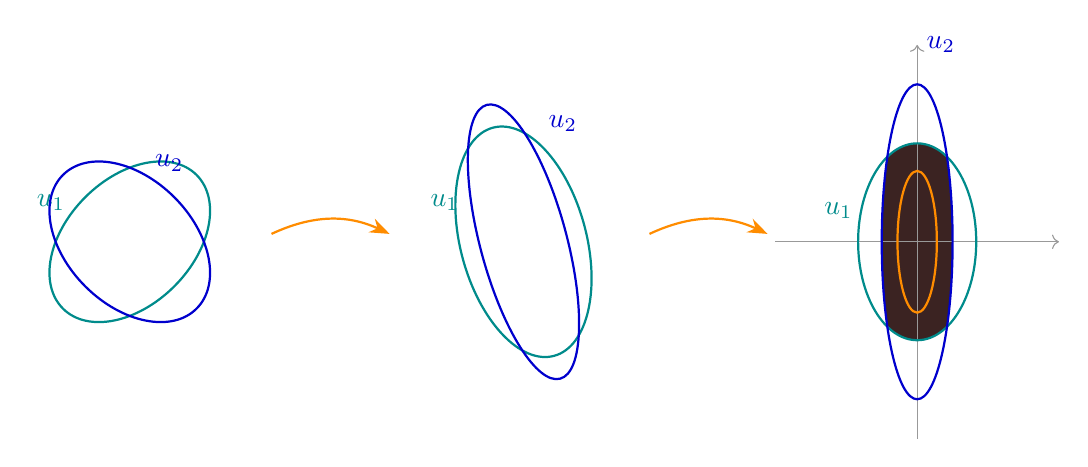
\begin{tikzpicture}

% Define custom colors to match the image
\definecolor{mygreen}{HTML}{008B8B} % DarkCyan, similar to teal
\definecolor{myblue}{HTML}{0000CD}  % MediumBlue
\definecolor{myorange}{HTML}{FF8C00} % DarkOrange
\definecolor{mydarkfill}{HTML}{3B2322} % A dark brown/black

% Part 1: Initial state
\begin{scope}[shift={(0,0)}]
    \draw[mygreen, thick, rotate=45] (0,0) ellipse (1.2 and 0.8);
    \node[mygreen] at (-1, 0.5) {$u_1$};
    \draw[myblue, thick, rotate=45] (0,0) ellipse (0.8 and 1.2);
    \node[myblue] at (0.5, 1) {$u_2$};
\end{scope}

% Arrow 1
\draw[-{Stealth[length=2.5mm]}, myorange, thick] (1.8, 0.1) to[bend left=25] (3.3, 0.1);

% Part 2: Intermediate state
\begin{scope}[shift={(5, 0)}]
    \draw[mygreen, thick, rotate=15] (0,0) ellipse (0.8 and 1.5);
    \node[mygreen] at (-1, 0.5) {$u_1$};
    \draw[myblue, thick, rotate=15] (0,0) ellipse (0.55 and 1.8);
    \node[myblue] at (0.5, 1.5) {$u_2$};
\end{scope}

% Arrow 2
\draw[-{Stealth[length=2.5mm]}, myorange, thick] (6.6, 0.1) to[bend left=25] (8.1, 0.1);

% Part 3: Final state
\begin{scope}[shift={(10, 0)}]
    \node[mygreen] at (-1, 0.4) {$u_1$};
    \node[myblue] at (0.3, 2.5) {$u_2$};

    % Define ellipses for reuse
    \def\ellipseA{(0,0) ellipse (0.75 and 1.25)} % Green
    \def\ellipseB{(0,0) ellipse (0.45 and 2.0)} % Blue

    % Fill intersection
    \begin{scope}
        \clip \ellipseA;
        \fill[mydarkfill] \ellipseB;
    \end{scope}

    % Axes
    \draw[->, gray!80] (-1.8, 0) -- (1.8, 0);
    \draw[->, gray!80] (0, -2.5) -- (0, 2.5);

    % Draw outer ellipse outlines
    \draw[mygreen, thick] \ellipseA;
    \draw[myblue, thick] \ellipseB;

    % Draw inner orange ellipse outline
    \draw[myorange, thick] (0,0) ellipse (0.25 and 0.9);
\end{scope}

\end{tikzpicture}
\end{document}
